\documentclass[../main/main.tex]{subfiles}
\graphicspath{{./figures/}}

\dominitoc
\faketableofcontents

\makeatletter
\renewcommand{\@chapapp}{Travaux pratiques -- TP}
\makeatother

% \toggletrue{student}
% \HideSolutionstrue

\begin{document}
\setcounter{chapter}{-1}

\chapter{Mesures et incertitudes}

\vfill

\begin{prgm}
	\begin{tcb}*(ror)"know"{Savoirs}
		\begin{itemize}[label=$\diamond$, leftmargin=10pt]
			\item Identifier les incertitudes liées, par exemple, à l'opérateur-ice, à
			      l'environnement, aux instruments ou à la méthode de mesure.
			\item Associer un intervalle de confiance à l'écart-type dans l'hypothèse
			      d'une distribution suivant la loi normale.
			\item Écrire, avec un nombre adapté de chiffres significatifs, le résultat
			      d’une mesure.
		\end{itemize}
	\end{tcb}

	\begin{tcb}*(ror)"how"{Savoir-faire}
		\begin{itemize}[label=$\diamond$, leftmargin=10pt]
			\item Procéder à l'évaluation d'une incertitude-type par une approche
			      statistique (type A).
			\item Procéder à l'évaluation d'une incertitude-type par une approche
			      autre que statistique (type B).
			\item Évaluer l'incertitude-type d'une grandeur s'exprimant en fonction
			      d'autres grandeurs, dont les incertitudes-types sont connues, à
			      l'aide d'une somme, d'une différence, d'un produit ou d'un quotient.
			\item Comparer deux valeurs dont les incertitudes-types sont connues à
			      l'aide de leur écart normalisé.
			\item Analyser les causes d’une éventuelle incompatibilité entre le
			      résultat d’une mesure et le résultat attendu par une modélisation
			      % \item Simuler, à l'aide d'un langage de programmation ou d'un tableur,
			      % un processus aléatoire permettant de caractériser la variabilité de la
			      % valeur d'une grandeur composée.
		\end{itemize}
	\end{tcb}
\end{prgm}

\vfill
\minitoc
\vfill

\newpage

% Pris de Maxime Champion - www.mchampion.fr

\section{Variabilité et incertitude-type}
\subsection{Variabilités de mesures}
Une expérience de mesure en science expérimentale est un processus généralement
complexe qui entremêle de très nombreux processus. Cette complexité se traduit
systématiquement par une variabilité de la mesure, qui implique que la
répétition de l'ensemble de la mesure conduit généralement à une valeur mesurée
sensiblement différente de la première. Cette variabilité est naturelle et fait
intrinsèquement partie de la mesure. Il ne faut pas chercher à la faire
disparaître, bien au contraire, elle renferme généralement une grande richesse
d'information sur le processus physique~!

Cette variabilité peut provenir de nombreux aspects, dont les principaux sont
les suivants :
\begin{itemize}[label=$\diamond$, leftmargin=10pt]
	\item la méthode de mesure~: règle graduée ou pied à coulisse pour une
	      longueur~;
	\item les variations de l'environnement~: célérité du son différente s'il fait
	      chaud ou froid~;
	\item les instruments de mesure~: deux voltmètres \textit{a priori} identiques
	      peuvent donner des résultats différents~;
	\item le processus physique même~: expériences de mécanique quantique, par
	      essence probabiliste~;
	\item l'expérimentataire.
\end{itemize}

\subsection{Incertitude-type}
\begin{tcb}[sidebyside, righthand ratio=.3](defi){Définition}
	La variabilité d'une mesure $x_{\rm exp}$ sur une grandeur $x$ est appelée
	\textbf{incertitude-type}, et se note $u(x_{\rm exp})$. Elle correspond
	mathématiquement à l'écart-type de la distribution qui surviendrait de mesures
	répétées.
	\tcblower
	Il est utile de définir l'incertitude-type \textbf{relative}, en
	pourcentages~:
	\[
		\boxed{u_r(x_{\rm exp}) = \frac{u(x_{\rm exp})}{x_{\rm exp}}}
	\]
\end{tcb}
\begin{figure}[htbp]
	\centering
	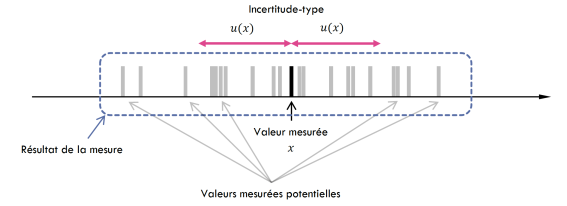
\includegraphics[scale=1]{inctype}
	\caption{Représentation d'un résultat de mesure expérimentale et du rôle de
		l'incertitude-type.}
	\label{fig:inctype}
\end{figure}
On notera que cette incertitude-type rend compte de toutes les grandeurs
d'influence possibles.

\begin{tcb}[sidebyside, lefthand ratio=.4](impo){Présentation d'un résultat de
			TP}
	Le résultat numérique d'une grandeur $x$ s'écrit~:
	\[
		\boxed{x = \left(x_{\rm exp} \pm u(x_{\rm exp})\right) \, \text{unité}}
	\]
	$x_{\rm exp}$ est la valeur \textbf{mesurée}, la meilleure estimation possible
	de la grandeur mesurée.
	\tcblower
	Par convention,
	\begin{itemize}[label=$\diamond$, leftmargin=10pt]
		\item Une incertitude-type comporte 2 chiffres significatifs~;
		\item Le dernier chiffre significatif de la mesure correspond à celui de
		      l'incertitude~:
		      \[
			      d = \SI{12.35\pm0.27}{m}
			      \quad \text{et pas} \quad
			      d = (\num{12.35}\cancel{2}\,\pm\,\num{0.27})\,\rm  m
		      \]
	\end{itemize}
\end{tcb}

\begin{tcb}(appl){Application}
	Corriger la présentation des valeurs suivantes, indiquer leur nombre de
	chiffres significatifs et calculer leurs incertitudes relatives $u_r$~:
	\[
		\lambda = \SI{589.0\pm11}{nm}
		\qquad
		t = \SI{0.473 \pm 0.122}{s}
		\qquad
		V = (14 \pm \num{0.0015})\,\si{mL}
	\]
	\tcblower
	\psw{
		On trouve
		\[
			\lambda = \SI{589\pm11}{nm}
			\qquad
			t = \SI{0.47 \pm 0.12}{s}
			\qquad
			V = \SI{14.0000 \pm 0.0015}{mL}
		\]
		avec respectivement 3, 2 et 6 chiffres significatifs. Pour les $u_r$, on trouve
		\[
			u_r(\lambda) = 1.9\%
			\qquad
			u_r(t) = 26\%
			\qquad
			u_r(V) = \num{0.011}\%
		\]
	}
\end{tcb}

\subsection{Comparaison de deux mesures}
Pour pouvoir comparer deux mesures entre elles, il faut un critère quantitatif
pour indiquer si ces deux mesures sont considérées comme compatibles ou
incompatibles.
\begin{tcb}(defi){Écart normalisé}
	L'\textbf{écart normalisé} $E_N$\ftn{Il est parfois appelé \textit{z-score},
		et noté $z$.} entre deux mesures de valeurs $x_1$ et $x_2$ et d'incertitudes
	$u(x_1)$ et $u(x_2)$ est défini par~:
	\[
		\boxed{E_N = \frac{\abs{x_1-x_2}}{\sqrt{u(x_1)^{2} + u(m_2)^{2}}}}
	\]
	Par \textit{convention}, on considère que \textbf{deux résultats sont
		compatibles si $E_N \lesssim 2$}.
\end{tcb}

\paragraph*{Interprétation}
Pour justifier cette convention, on peut revenir à la définition de
l'incertitude-type. Celle-ci quantifie les fluctuations potentielles de la
valeur mesurée annoncée. Lorsque deux mesures sont cohérentes, on s'attend à ce
qu'elles ne coïncident pas exactement, mais qu'elles ne s'écartent pas l'une de
l'autre de plus que de quelques incertitudes-type.

\begin{figure}[htbp]
	\centering
	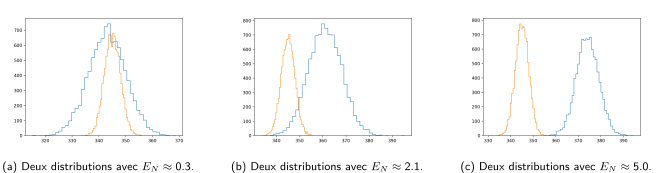
\includegraphics[scale=1]{zscore}
	\caption{Tracé de deux distributions de résultats de mesures.}
	\label{fig:zscore}
\end{figure}

\paragraph*{Comparaison avec une valeur de référence}
Dans le cas d'une valeur donnée sans incertitude, ou avec une incertitude
très faible comparée à la nôtre, $u(x_{\rm exp}) \gg u(x_{\rm ref})$ implique
donc
\[
	E_N = \frac{\abs{x_{\rm exp} - x_{\rm ref}}}{u(x_{\rm exp})}
\]

\paragraph*{En dépit d'incertitudes}
Si aucune des incertitudes n'est connue ou déterminée, on peut utiliser~:
\begin{tcolorbox}[blankest]
	\begin{isd}
		\tcbsubtitle{\fatbox{Écart absolu}}
		\[
			\ep = \abs{x_{\rm exp} - x_{\rm ref}}
			\vphantom{\abs{\frac{x_{\rm exp} - x_{\rm ref}}{x_{\rm ref}}}}
		\]
		\tcblower
		\tcbsubtitle{\fatbox{Écart relatif}}
		\[
			\ep_r = \abs{\frac{x_{\rm exp} - x_{\rm ref}}{x_{\rm ref}}}
		\]
	\end{isd}
\end{tcolorbox}

Cette notion n'est officiellement plus au programme mais reste utilisée dans
certains sujets.

\section{Estimation pour une mesure variable~: type A}

Lorsque l'on réalise plusieurs fois et de manière indépendante une mesure, il
est possible d'évaluer statistiquement la mesure. Ainsi, pour $n$ mesures notées
$x_i$~:
\begin{enumerate}
	\item on définit $\obar{x} = x_{\rm exp}$ la \textbf{moyenne} de
	      l'ensemble avec~:
	      \[
		      \obar{x} = x_{\rm exp} = \frac{1}{n} \sum_{i=1}^{n} x_i
	      \]
	\item et l'incertitude-type sur \textbf{UNE MESURE} $x_i$
	      \[
		      u(x_i) = \sigma =
		      \sqrt{\frac{1}{n-1} \sum_{i=1}^{n} (x_i - \obar{x})^{2}}
	      \]
	      Attention, selon les logiciels ou calculatrices, c'est $n$ au lieu $n-1$~!
	      Notamment pour les Casio, \texttt{$\sigma x$} est la version non désirée, et
	      \texttt{sx} est la version avec $n-1$ comme attendu. On notera quoiqu'il en soit
	      que cette incertitude-type est la même pour \xul{toutes} les mesures $x_i$, par
	      construction.
\end{enumerate}
Le fait de répéter un grand nombre de fois une mesure \textit{réduit}
l'incertitude associée à la moyenne, puisque les fluctuations supposées
aléatoires se compensent. Ainsi,
\begin{enumerate}[resume]
	\item l'incertitude-type sur \textbf{LA MOYENNE} $x_{\rm exp}$ réduit avec le
	      nombre de mesures, tel que
	      \[
		      u(\obar{x}) = \frac{u(x_i)}{\sqrt{n}} = \frac{\sigma}{\sqrt{n}}
	      \]
\end{enumerate}

On remarquera que le procédé n'est pas linéaire~: pour avoir une incertitude 10
fois plus faible, il faut 100 fois plus de mesures~!

\begin{tcb}(ror)<fil>{Incertitude de type A}
	Pour $n$ mesures $x_i$,
	\smallbreak
	\begin{isd}[cnt](ror)
		\tcbsubtitle{\fatbox{Valeur mesurée}}
		C'est la moyenne des mesures.
		\[
			\boxed{x_{\rm exp} = \obar{x} = \frac{1}{n} \sum_{i=1}^{n} x_i}
		\]
		\tcblower
		\tcbsubtitle{\fatbox{Incertitude}}
		C'est l'écart-type divisé par $\sqrt{n}$.
		\[
			\boxed{u(\obar{x}) = \frac{\sigma}{\sqrt{n}}}
		\]
	\end{isd}
\end{tcb}

\begin{tcb}(appl){Application}
	On a obtenu par dosage rédox le degré d'alcool d'un vin à 8 reprises. Les
	mesures ont donné~:
	\begin{center}
		\begin{tabular}{lcccccccc}
			\toprule
			Degré ($\si{\degree}$) &
			\num{11.9}             &
			\num{12.5}             &
			\num{13.1}             &
			\num{12.4}             &
			\num{12.9}             &
			\num{12.6}             &
			\num{12.8}             &
			\num{12.6}
			\\
			\bottomrule
		\end{tabular}
	\end{center}
	À l'aide de votre calculatrice, d'un tableur ou d'un script \texttt{Python},
	exprimer le résultat de ces mesures ainsi que son incertitude.
	\tcblower
	\begin{python}
		import numpy as np

		vals = np.array([11.9, 12.5, 13.1, 12.4, 12.9, 12.6, 12.8, 12.6])
		mean = np.mean(vals)
		ecarttype = np.std(vals, ddof=1)
		incertype = ecarttype/np.sqrt(len(vals))
		print(f'D = {mean:.2f} +- {incertype:.2f}')
	\end{python}
	On trouve
	\[
		\xul{
			\psw{
				D = \SI{12.60 \pm  0.13}{\degree}
			}
		}
	\]
\end{tcb}

\section{Estimation pour une mesure invariable~: type B}

Lorsque qu'il est impossible (\textit{pas de variabilité observée de la
	mesure}), ou trop long, de faire une évaluation de type A, l'incertitude est
alors évaluée à l'aide de connaissances préalables sur le dispositif
expérimental~: mesures antérieures, spécifications du fabricant, expérience ou
connaissances du comportement ou des propriétés des instruments utilisés.
\bigbreak
\noindent
\begin{minipage}[t]{.50\linewidth}
	Dans beaucoup de cas, il est possible d'estimer le plus petit intervalle dans
	lequel on est certain-e trouver toutes les valeurs possibles de $x$. On note
	$x_c$ la valeur centrale de cet intervalle.
	\smallbreak
	En l'absence d'autre information sur la variabilité, on attribue une
	\textit{loi de probabilité rectangulaire} à la mesure (équiprobabilité des
	mesures dans l'intervalle de largeur $2\Delta$) et on calcule l'écart-type de
	la distribution rectangulaire de demi-largeur $\Delta$~:
\end{minipage}
\hfill
\begin{minipage}[t]{.45\linewidth}
	~
	\vspace*{-10pt}
	\begin{center}
		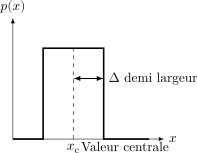
\includegraphics[scale=1]{typeB}
		\label{fig:typeB}
	\end{center}
\end{minipage}
\[
	\boxed{u(x) = \frac{\Delta}{\sqrt{3}}}
\]

On a trois cas de figures courant pour la mesure de $\Delta$~:
\begin{enumerate}
	\item $\Delta$ est égale à \textbf{une graduation} de l'appareil~;
	\item $\Delta$ est fournie sur la notice~;
	\item $\Delta$ est estimée directement avec honnêteté.
\end{enumerate}

\begin{tcb}(ror)<fil>{Incertitude de type B}
	Pour une mesure invariable,
	\smallbreak
	\begin{isd}[cnt](ror)
		\tcbsubtitle{\fatbox{Valeur mesurée}}
		C'est la valeur centrale de l'intervalle.
		\[
			\boxed{x_{\rm exp} = x_c}
		\]
		\tcblower
		\tcbsubtitle{\fatbox{Incertitude}}
		C'est la demi-largeur de l'intervalle divisé par $\sqrt{3}$.
		\[
			\boxed{u(x_c) = \frac{\Delta}{\sqrt{3}}}
		\]
	\end{isd}
\end{tcb}

\begin{tcb}(appl){Application}
	Évaluer les incertitudes et donnez les résultats des expériences suivantes~:
	\begin{enumerate}
		\item Mesure d'une longueur $\ell = \SI{13}{cm}$ avec une règle graduée au
		      \si{mm}.
		      \smallbreak
		      \psw{
			      Largeur = \SI{1}{mm} = \SI{0.1}{cm}, donc
			      \[
				      \xul{\ell = \SI{13.000 \pm 0.058}{cm}}
			      \]
		      }
		      \vspace*{-20pt}
		\item Utilisation d'un multimètre pour mesurer une tension $U$. Il affiche
		      \SI{2.5462}{V} et la notice indique \textit{Accuracy=0.3\% rdg + 2
			      digits}, autrement dit de \num{0.3}\% de la valeur lue (\textit{rdg} =
		      \textit{reading}) auquel on ajoute 2 fois la valeur du dernier chiffre.
		      \smallbreak
		      \psw{
			      On trouve $u(U) = \SI{0.0080}{V}$, d'où
			      \[
				      \xul{U = \SI{2.5462 \pm 0.0080}{V}}
			      \]
		      }
		      \vspace*{-20pt}
		\item Mesure de la position $d$ d'un écran sur un banc optique. L'image
		      semble nette pour des positions allant de \num{29.7} à \SI{30.5}{cm}.
		      \smallbreak
		      \psw{
			      On a
			      \[
				      x_c = \SI{30.1}{cm}
				      \qet
				      \Delta = \SI{0.40}{cm}
				      \qdc
				      \xul{d = \SI{30.10 \pm 0.23}{cm}}
			      \]
		      }
		      \vspace*{-20pt}
	\end{enumerate}
\end{tcb}

\section{Incertitudes composées}
Dans de très nombreuses situations, on est amené à calculer la valeur d'une
grandeur à partir de valeurs mesurées et donc possédant des incertitudes.
Comment exprimer alors l'incertitude sur ce calcul en fonction de celles sur les
données utilisées ?

\subsection{Calcul à partir d'une seule valeur mesurée}
\[
	\boxed{y_{\rm calc} = f(x_{\rm mes}) \Ra u(y_{\rm calc}) =
		\abs{\dv{f}{x}(x_{\rm mes})}u(x_{\rm mes})}
\]

\begin{tcb}[breakable](appl){Application}
	On envoie une impulsion laser de la Terre sur la Lune. On mesure son
	aller-retour en $t = \SI{2.57 \pm 0.02}{s}$. Sachant que la célérité de la
	lumière dans le vide est exactement $c = \SI{299792458}{m.s^{-1}}$, déterminer
	la distance Terre-Lune (qu'on nommera $d$) ainsi que son incertitude.
	\tcblower
	\vspace*{-10pt}
	\begin{isd}
		\psw{L'impulsion parcourt $2d$ en $t$ à la vitesse $c$. Ainsi,
			\[
				\boxed{d = \frac{c}{2}t}
				\quad \Ra \quad
				\abs{\dv{\left(\frac{c}{2}t\right)}{t}} = \frac{c}{2}
			\]
		}
		\vspace*{-10pt}
		\tcblower
		\psw{
			Ainsi, par A.N.,
			\begin{gather*}
				d = \SI{385344308.5 \pm 2997924.58}{m}
				\\\Ra
				\xul{d = \SI{3.853 \pm 0.030e5}{km}}
				\\\Ra
				\xul{d= \SI{385.3 \pm 3.0e3}{km}}
			\end{gather*}
		}
		\vspace*{-10pt}
	\end{isd}
\end{tcb}

\subsection{Calcul avec deux valeurs mesurées (\textit{à connaître})}
\begin{tcb}(ror){Incertitudes composées à 2 variables}
	\tcbsubtitle{\fatbox{Somme ou différence}}
	\[
		\boxed{
			y = x_1 \pm x_2
			\qquad \Ra \qquad
			u(y) = \sqrt{(u(x_1))^{2} + (u(x_2))^{2}}}
	\]
	\tcblower
	\tcbsubtitle{\fatbox{Produit de puissances}}
	\[
		\boxed{
		y = x_1^{\alpha_1}x_2^{\alpha_2}
		\qquad \Ra \qquad
		\frac{u(y)}{y} = \sqrt{
			\abs{\alpha_1}\left(\frac{u(x_1)}{x_1}\right)^{2} +
			\abs{\alpha_2}\left(\frac{u(x_2)}{x_2}\right)^{2}
		}
		}
	\]
\end{tcb}

\begin{tcb}(appl){Application}
	On mesure la distance $d = x_2 - x_1$ entre deux points repérés avec la même
	incertitude $u(x_1) = u(x_2) = \SI{1}{mm}$. Quelle est l'incertitude sur $d$~?
	\smallbreak
	\psw{
		On trouve élémentairement~:
		\[
			u(d) = \sqrt{1+1} = \SI[parse-numbers=false]{\sqrt{2}}{mm}
		\]
	}
	\tcblower
	On détermine la célérité $c$ du son dans l'air grâce à la relation $\lambda =
		\frac{c}{f}$, avec $f = \SI{500 \pm 10}{Hz}$ et $\lambda = \SI{68.0 \pm
			2.5}{cm}$. Donner sa valeur.
	\smallbreak
	\psw{
		On trouve
		\[
			\xul{c = \SI{340 \pm 14}{m.s^{-1}}}
		\]
	}
\end{tcb}

\subsection{Incertitudes-types composées quelconques}
Seules les deux formules précédentes sont à connaître, pour tous les autres cas,
nous allons revenir à la définition des incertitudes puis, à l'aide d'une
simulation informatique comportant une part d'aléatoire, calculer
l'incertitude-type. Une fiche y sera consacrée.
\begin{tcb}(defi){Définition}
	Un algorithme utilisant la variabilité d'une mesure pour simuler un calcul
	d'incertitude fait parti des algorithmes de type \textsc{Monte-Carlo}.
\end{tcb}
\end{document}
